% This is a Basic Assignment Paper but with like Code and stuff allowed in it, there is also url, hyperlinks from contents included. 

\documentclass[11pt]{article}

% Preamble

\usepackage[margin=1in]{geometry}
\usepackage{amsfonts, amsmath, amssymb}
\usepackage{fancyhdr, float, graphicx}
\usepackage[utf8]{inputenc} % Required for inputting international characters
\usepackage[T1]{fontenc} % Output font encoding for international characters
\usepackage{fouriernc} % Use the New Century Schoolbook font
\usepackage[nottoc, notlot, notlof]{tocbibind}
\usepackage{listings}
\usepackage{xcolor}
\usepackage{blindtext}
\usepackage{hyperref}
\hypersetup{
    colorlinks=true,
    linkcolor=black,
    filecolor=magenta,      
    urlcolor=cyan,
    pdfpagemode=FullScreen,
    }

\definecolor{codegreen}{rgb}{0,0.6,0}
\definecolor{codegray}{rgb}{0.5,0.5,0.5}
\definecolor{codepurple}{rgb}{0.58,0,0.82}
\definecolor{backcolour}{rgb}{0.95,0.95,0.92}

\lstdefinestyle{mystyle}{
    backgroundcolor=\color{backcolour},   
    commentstyle=\color{codegreen},
    keywordstyle=\color{magenta},
    numberstyle=\tiny\color{codegray},
    stringstyle=\color{codepurple},
    basicstyle=\ttfamily\footnotesize,
    breakatwhitespace=false,         
    breaklines=true,                 
    captionpos=b,                    
    keepspaces=true,                 
    numbers=left,                    
    numbersep=5pt,                  
    showspaces=false,                
    showstringspaces=false,
    showtabs=false,                  
    tabsize=2
}

\lstset{style=mystyle}

% Header and Footer
\pagestyle{fancy}
\fancyhead{}
\fancyfoot{}
\fancyhead[L]{\textit{\Large{Philosophy of Science and Religion - Second Year B. Tech, Semester 2}}}
%\fancyhead[R]{\textit{something}}
\fancyfoot[C]{\thepage}
\renewcommand{\footrulewidth}{1pt}



% Other Doc Editing
% \parindent 0ex
%\renewcommand{\baselinestretch}{1.5}

\begin{document}

\begin{titlepage}
	\centering

	%---------------------------NAMES-------------------------------

	\huge\textsc{
		MIT World Peace University
	}\\

	\vspace{0.75\baselineskip} % space after Uni Name

	\LARGE{
		Philosophy of Science and Religion\\
		Second Year B. Tech, Semester 1
	}

	\vfill % space after Sub Name

	%--------------------------TITLE-------------------------------

	\rule{\textwidth}{1.6pt}\vspace*{-\baselineskip}\vspace*{2pt}
	\rule{\textwidth}{0.6pt}
	\vspace{0.75\baselineskip} % Whitespace above the title



	\huge{\textsc{
			Film Review\\
			\textit{"English Vinglish"}
		}} \\



	\vspace{0.5\baselineskip} % Whitespace below the title
	\rule{\textwidth}{0.6pt}\vspace*{-\baselineskip}\vspace*{2.8pt}
	\rule{\textwidth}{1.6pt}

	\vspace{1\baselineskip} % Whitespace after the title block

	%--------------------------SUBTITLE --------------------------	

	\LARGE\textsc{
		Film Review
	} % Subtitle or further description
	\vfill

	%--------------------------AUTHOR-------------------------------

	Prepared By
	\vspace{0.5\baselineskip} % Whitespace before the editors

	\Large{
		Krishnaraj Thadesar \\
		Cyber Security and Forensics\\
		Batch A1, PA 20
	}


	\vspace{0.5\baselineskip} % Whitespace below the editor list
	\today

\end{titlepage}


\tableofcontents
\thispagestyle{empty}
\clearpage

\setcounter{page}{1}

% Sections
% 1. Name of the Film
% 2. Theme of the Film (Social, Environmental, Patriotic etc.)
% 3. Main Character
% 4. Social Impact
% 5. Learning / take away from Film
% 6. Your critical evaluation of Film (what could have been better)
% 7. Your rating about film

\section{Name of the Film}

\subsection*{English Vinglish}

\begin{figure}[H]
    \centering
    
\includegraphics[width=.45\textwidth]{English_Vinglish_poster.jpg}
    \caption{English Vinglish Poster}
\end{figure}
\textit{English Vinglish is a 2012 Indian comedy-drama film directed by Gauri Shinde. The film marked the comeback of the legendary actress Sridevi after a hiatus of 15 years. The film was widely appreciated for its subtle humor and realistic portrayal of the struggles faced by women in India. English Vinglish was released in several languages across the world and was a commercial and critical success. The film's music, composed by Amit Trivedi, was also well received, with the song "Navrai Majhi" becoming a popular wedding song.}


\section{Theme of the Film}

The theme of the film English Vinglish is centered around self-discovery, identity, and self-esteem. The film challenges the societal norms and perceptions that equate fluency in English with intelligence and success. Shashi's struggle to learn English and the way she is ridiculed by her family members for her inability to speak the language is a common experience for many women in India.\\

The film highlights the importance of self-confidence and self-worth, which are often undermined by societal pressures and expectations. The film also touches upon the theme of cultural identity, as Shashi learns to appreciate her mother tongue and cultural heritage through her interactions with the diverse people she meets in New York.

\begin{figure}[H]
    \centering
    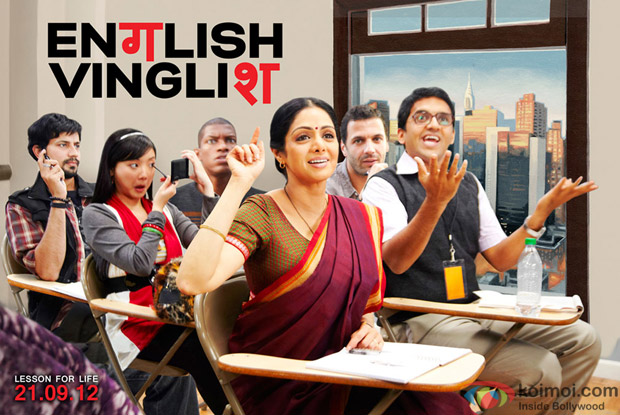
\includegraphics[width=.45\textwidth]{English-Vinglish-Movie-Review.jpg}
    \caption{English Vinglish Movie Review Poster}
\end{figure}


\section{Social Impact}

English Vinglish has had a significant social impact in India, where English is often seen as a symbol of status and success. The film has encouraged people to appreciate the value of their mother tongue and cultural heritage. It has also sparked a conversation about the importance of self-confidence and self-worth.\\

The film has been widely discussed and analyzed in academic circles, with many scholars praising its realistic portrayal of women's issues in India. The film has also inspired several other films and TV shows that explore similar themes.


\section{Main Character}

\subsection*{Shashi}


Shashi, played by Sridevi, is the heart and soul of the film English Vinglish. Shashi is a middle-aged Indian housewife who is dedicated to her family and runs a small business of making and selling ladoos from her home. Despite her many accomplishments, she is constantly belittled by her family for her inability to speak fluent English. \\

Shashi's character is relatable to many women in India who are often undervalued and undermined due to societal expectations and gender roles. Sridevi's portrayal of Shashi is nuanced and realistic, making her a memorable and endearing character.

\section{Learning / Take Away from Film}

The film English Vinglish teaches us several important lessons. Firstly, it shows us the importance of self-discovery and self-esteem. Shashi's journey of learning English and gaining confidence in herself is inspiring and relatable.\\

The film also highlights the importance of cultural identity and the need to appreciate one's mother tongue and cultural heritage. Secondly, the film challenges societal norms and perceptions that equate fluency in English with intelligence and success. The film encourages viewers to value their own skills and talents, regardless of their proficiency in a particular language.

\section{Critical Evaluation of Film}


While English Vinglish is an excellent film with a strong message, there are a few areas where the film could have been improved. The pacing of the film is uneven in some parts, with some scenes feeling stretched out. Additionally, some of the family members' behavior towards Shashi feels unrealistic and exaggerated. \\

The climax of the film could also have been more impactful if it had been given more time to develop. However, these minor flaws do not detract from the overall impact and quality of the film.


\section{Rating of Film}
is inspiring and relatable, and the performances by the cast, especially Sridevi, are outstanding. The film's subtle humor and realistic portrayal of Indian women's struggles have made it a cultural touchstone in India. It is a heartwarming and feel-good film that leaves a lasting impact on the audience.\\

On a scale of 1 to 10, I would give English Vinglish an 8. The film is well-directed, well-acted, and has a strong message that resonates with viewers. However, there are a few areas where the film could have been improved, such as the pacing and the portrayal of some of the family members. Nevertheless, the film's impact on Indian society and its positive portrayal of women's issues make it a must-watch film. Overall, English Vinglish is a film that will leave you with a smile on your face and a warm feeling in your heart.

\end{document}